%卒論概要テンプレート ver. 4.0

\documentclass[uplatex,twocolumn,dvipdfmx]{jsarticle}
\usepackage[top=22mm,bottom=22mm,left=22mm,right=22mm]{geometry}
\setlength{\columnsep}{11mm}
\usepackage[T1]{fontenc}
\usepackage{txfonts}
\usepackage[expert,deluxe]{otf}
\usepackage[dvipdfmx,hiresbb]{graphicx}
\usepackage[dvipdfmx]{hyperref}
\usepackage{pxjahyper}
\usepackage{secdot}

%タイトルと学生番号,名前だけ編集すること
\title{\vspace{-5mm}\fontsize{14pt}{0pt}\selectfont Twitter発言の分析によるWebサービス障害の影響調査}
\author{\normalsize プロジェクトマネジメントコース 矢吹研究室 1442012 岩瀬翔}
\date{}
\pagestyle{empty}
\begin{document}
\fontsize{10.5pt}{\baselineskip}\selectfont
\maketitle

%以下が本文
\section{序論}\label{序論}

複数のメンバが同時に開発を行うソフトウェア開発プロジェクトにおいて,「GitHub」のようなWebサービスが使われることがある.

Webサービスの停止は,それを利用しているプロジェクトに大きな影響を与えると思われる.実際,2016年1月28日のGitHubの停止時には,そのせいで仕事が進められなくなったというようなツイートがTwitter上で複数観測された\cite{01}.

\section{目的}

Twitterの発言を収集するためのツールを開発し,それを用いてソフトウェア開発で利用されるWebサービスの停止が開発に与える影響を調査する.

\section{手法}
2016年に発生したGitHubの障害発生に関するツイートをデータとして収集する.TwitterのAPIには,1週間以上前のツイートは取得できない制限がある\cite{02}.そこで,制限無く検索できるブラウザのTwitterを利用する.この検索結果は画面を最下部にスクロールすることで古いものが読み込まれていく.検索する日付はGitHubを継続的に監視している「GitHub Status」を参照する.

データを収集するツールを開発するために2つのプログラムを作成する.1つ目では,ブラウザの自動操作ができるライブラリである「Selenium WebDriver」を使用し,画面スクロール後,HTMLファイルを保存する.2つ目では,Pythonのライブラリである「BeautifulSoup4」でデータを抽出する.

\section{結果}
\vspace{-1.5zh}
\begin{figure}[htbp]
 \begin{tabular}{cc}
  \begin{minipage}{0.5\hsize}
    \begin{center}
      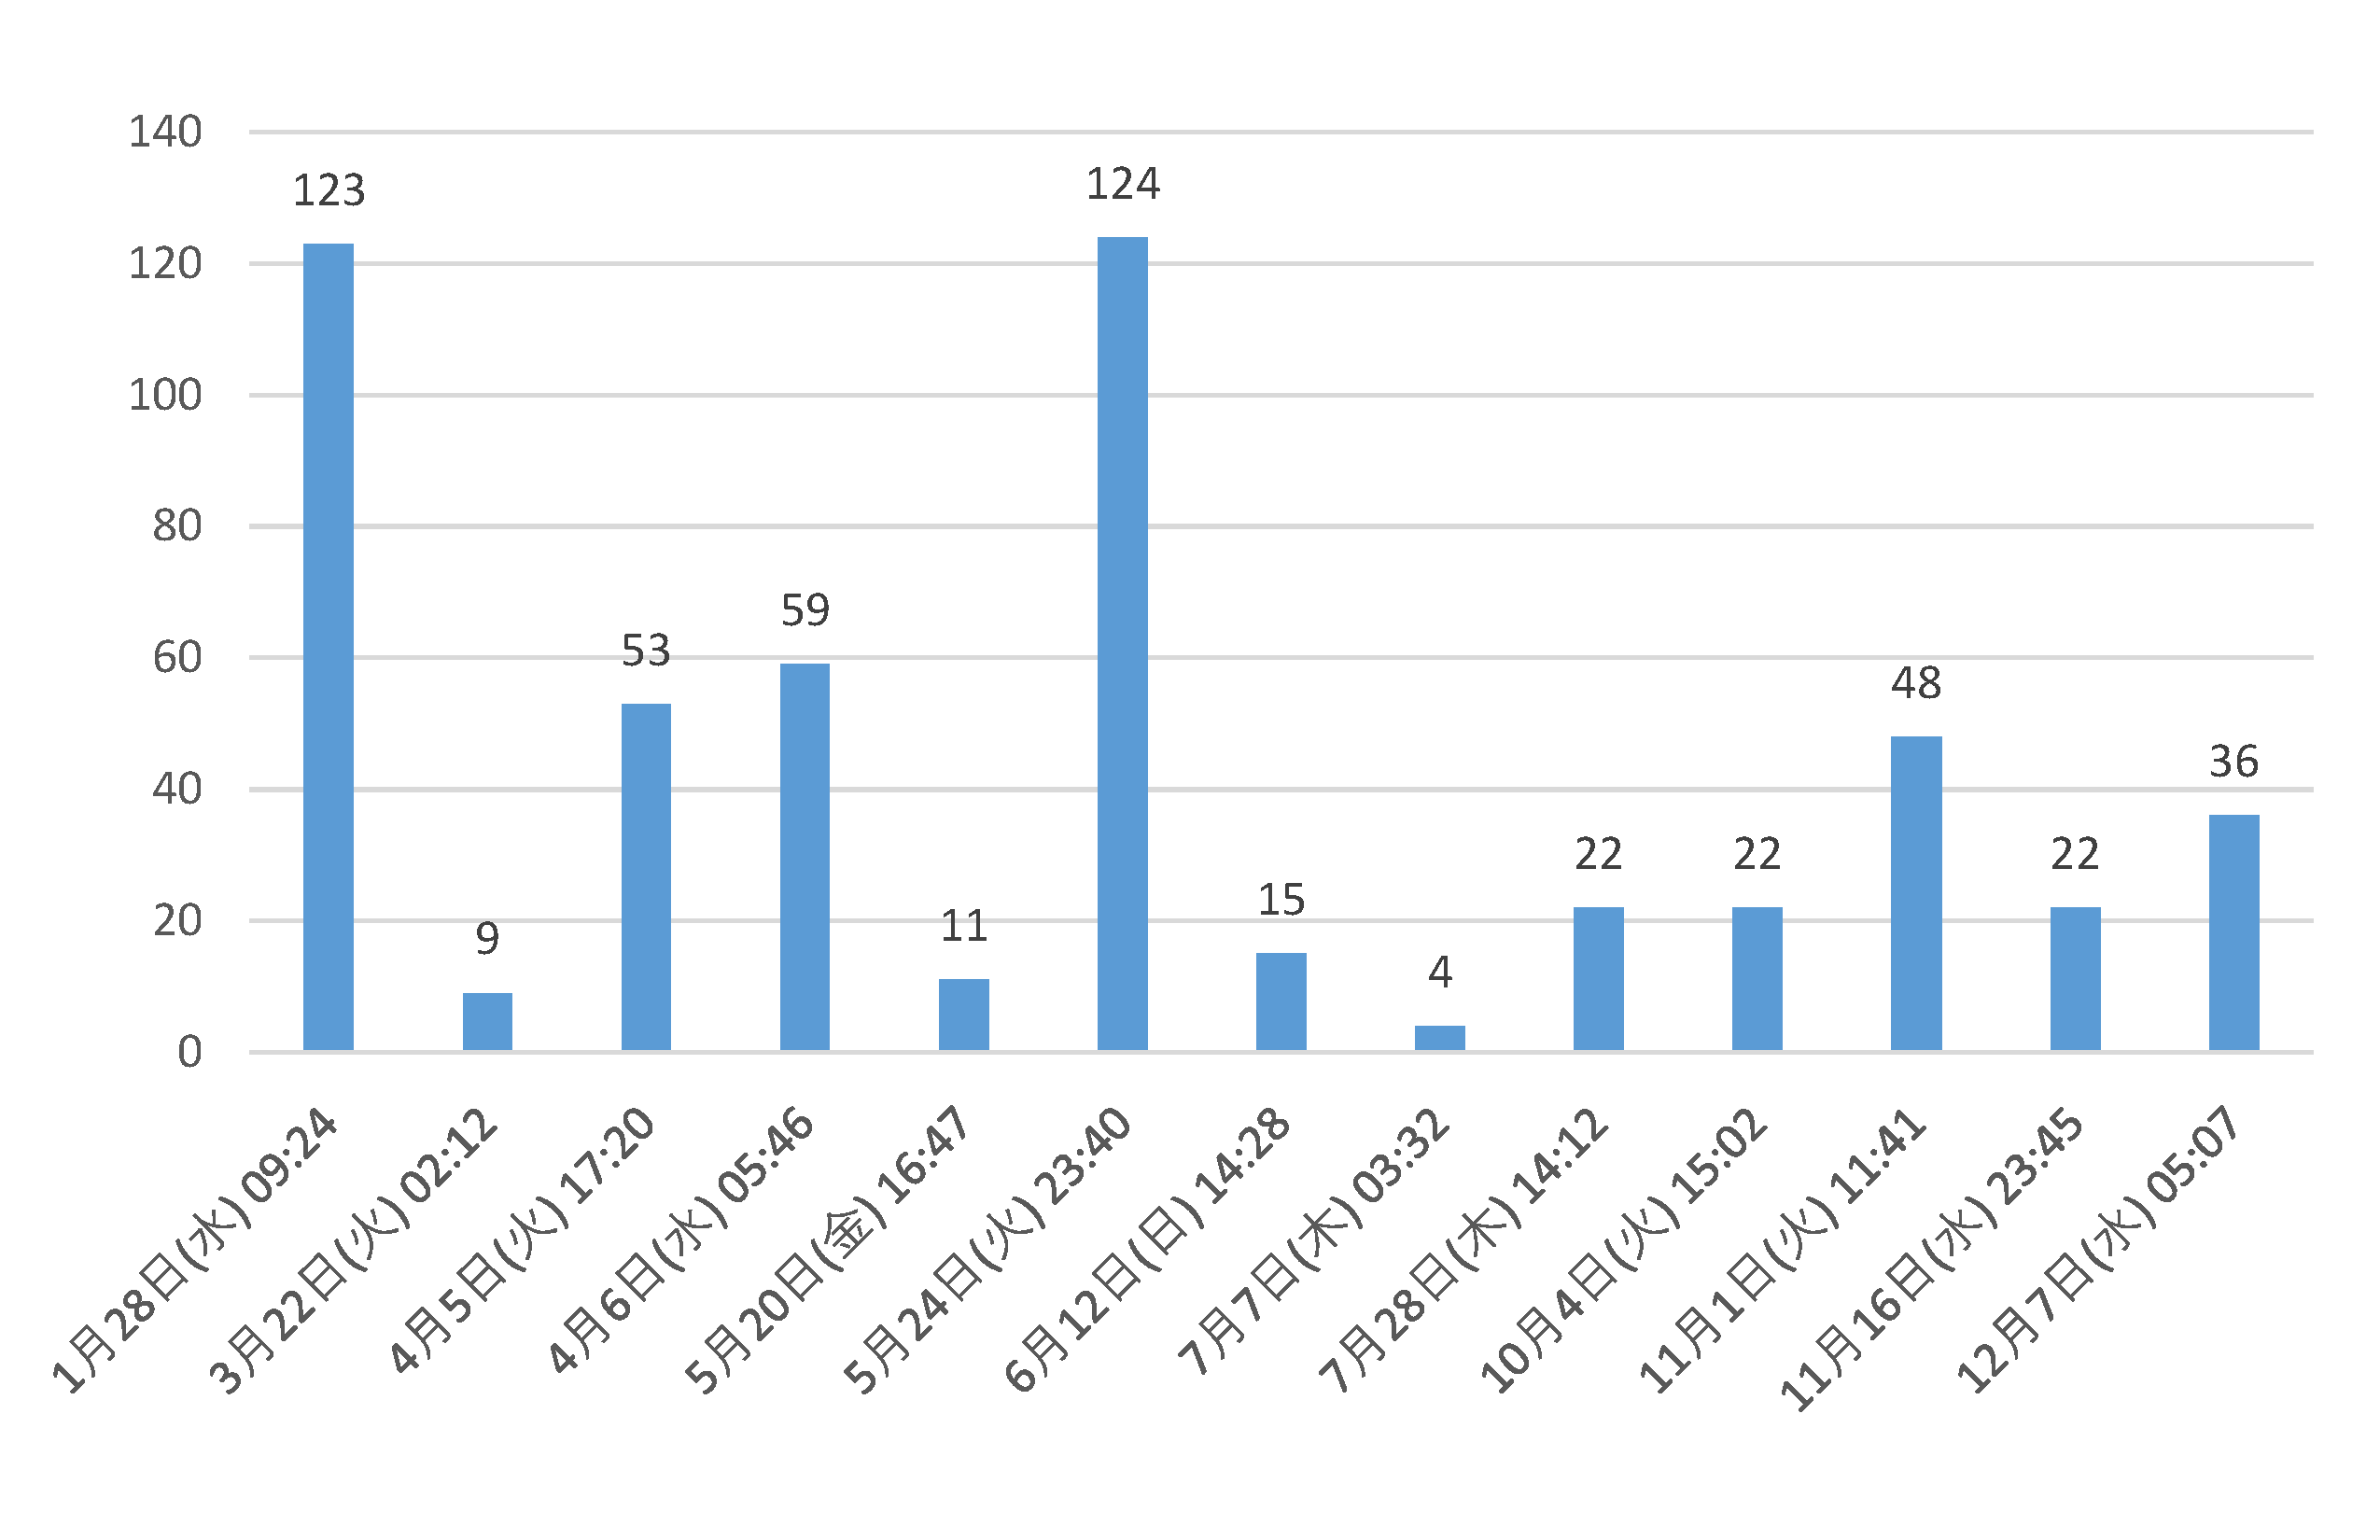
\includegraphics[width=38mm,clip]{graph1.pdf}
      \caption{サービス停止から復旧までの間隔}
      \label{時間}
  \end{center}
  \end{minipage}
  \begin{minipage}{0.5\hsize}
    \begin{center}
      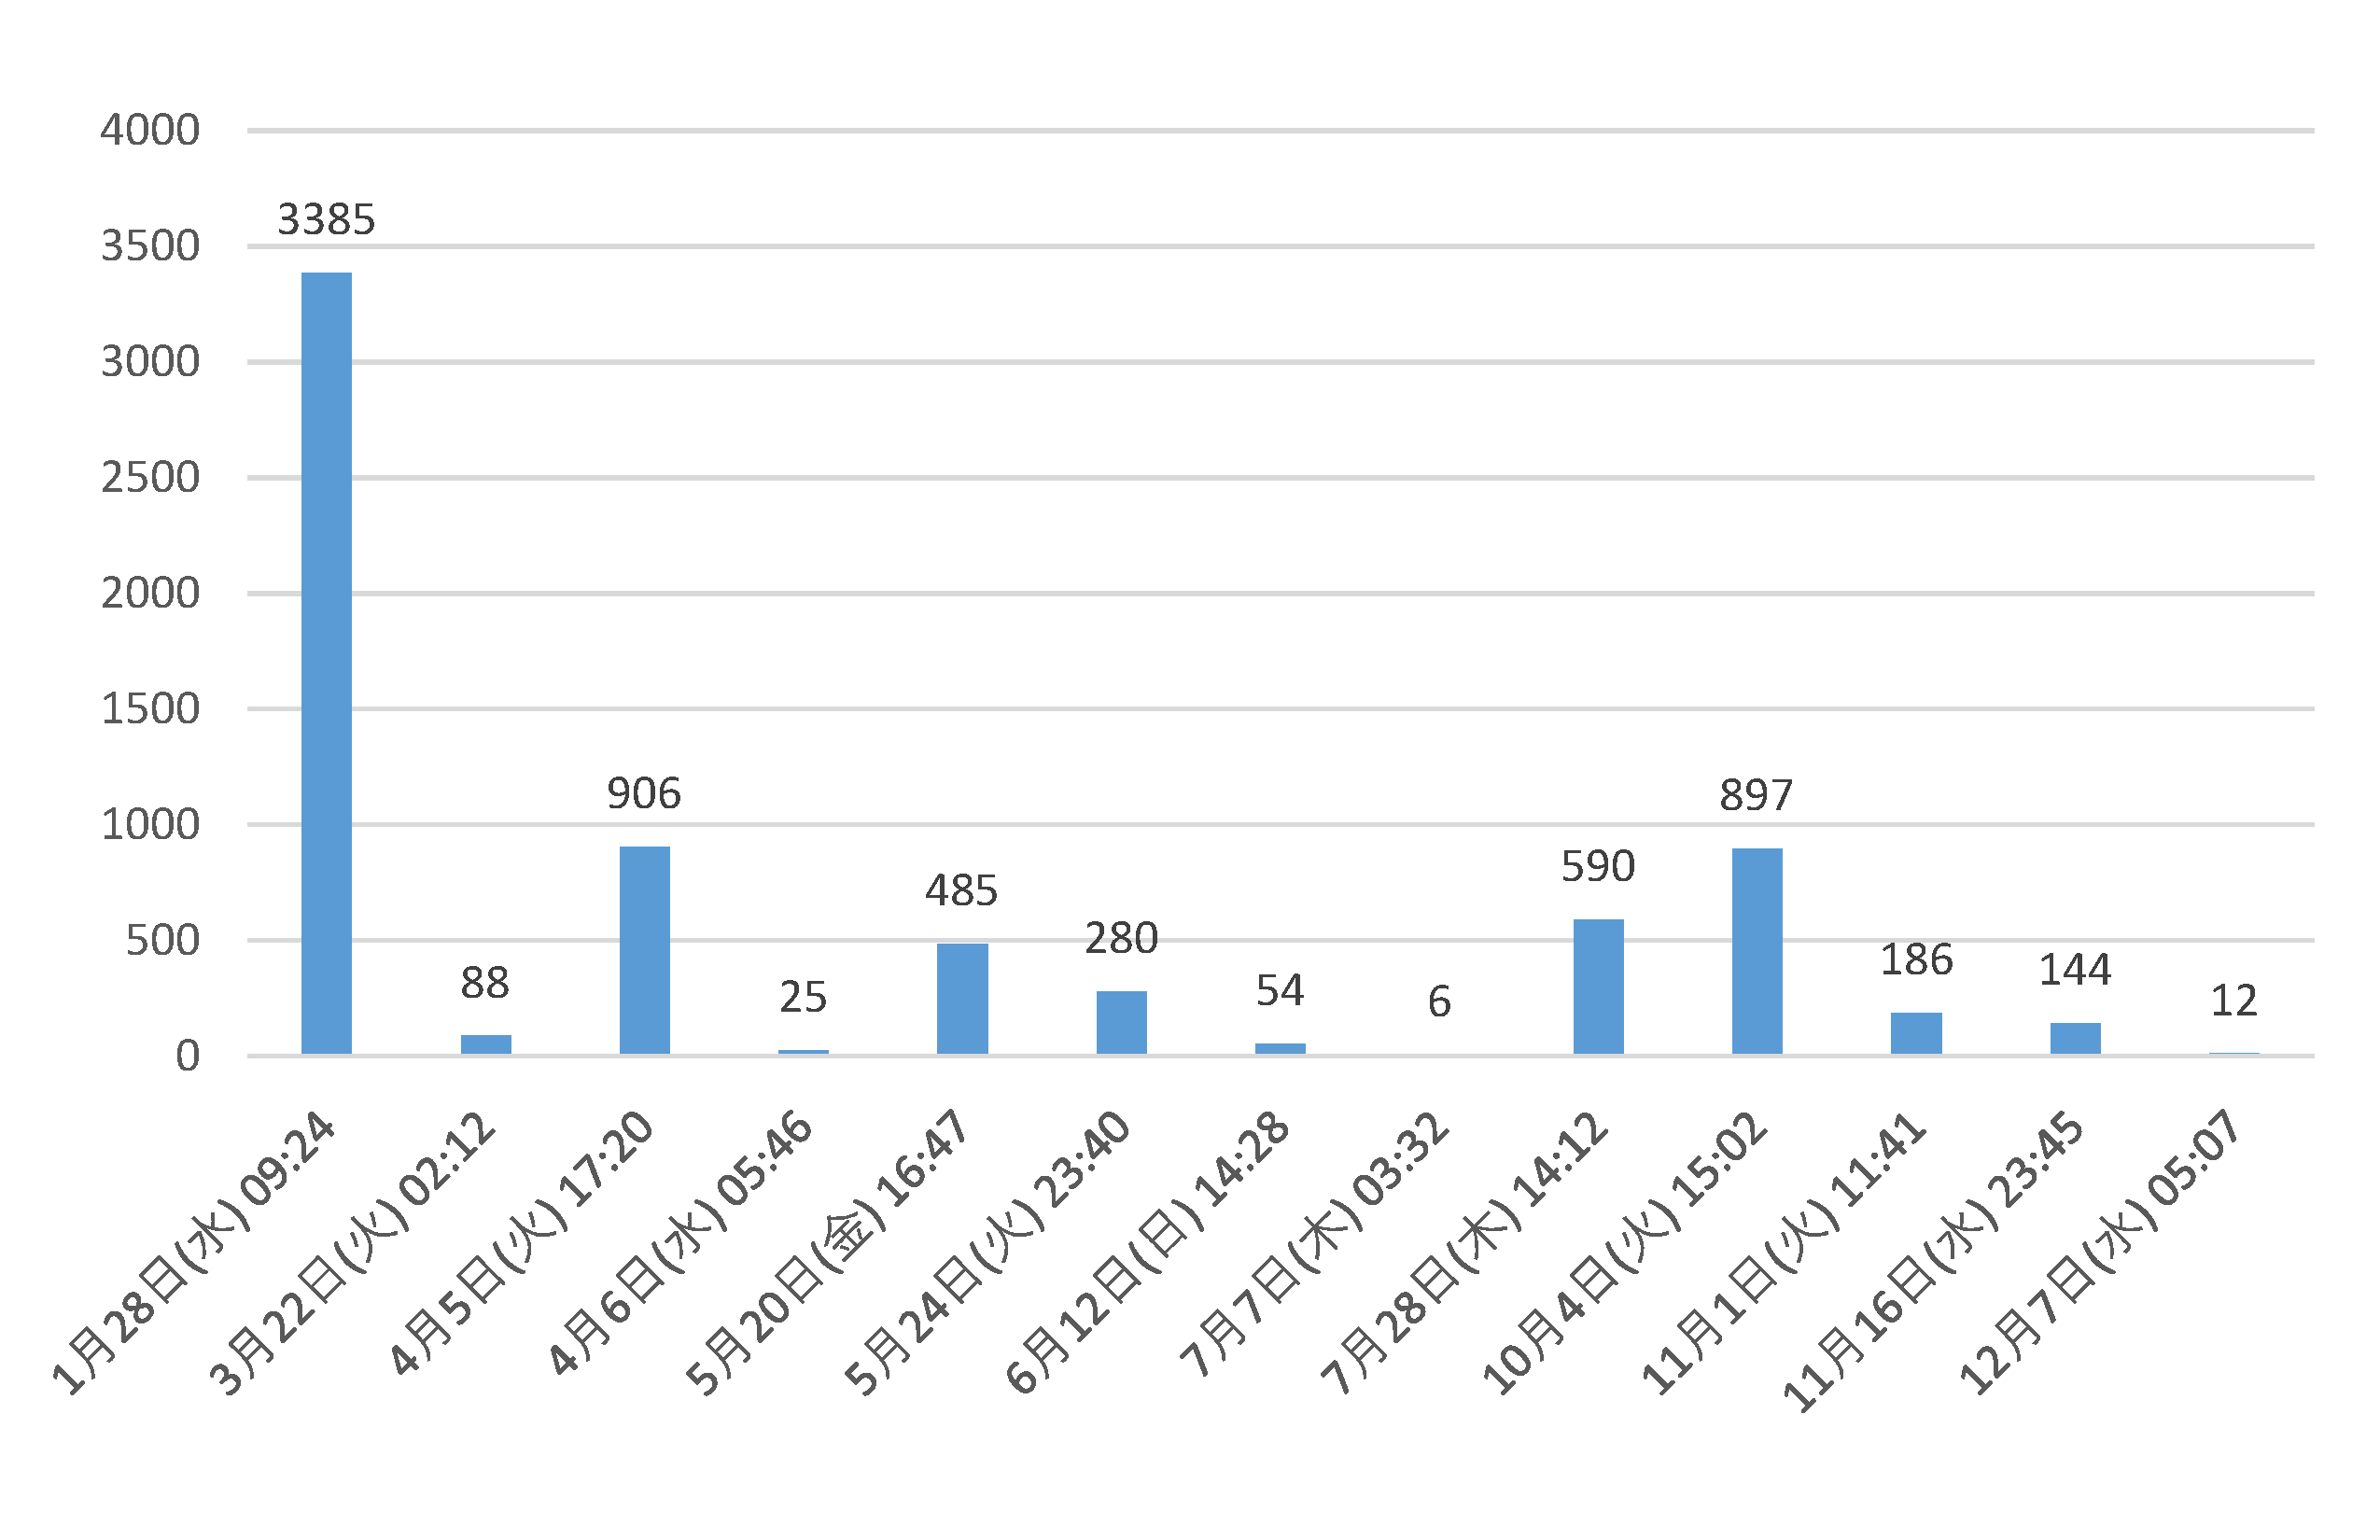
\includegraphics[width=38mm,clip]{graph2.pdf}
      \caption{サービス停止中に投稿されたツイートの数}
      \label{ツイート数}
   \end{center} 
  \end{minipage}
 \end{tabular}
\end{figure}
\vspace{-1.5zh}
2016年にGitHubで発生した13回のサービス停止を調査対象とする.
各障害のサービス停止から復旧までの間隔を分単位でグラフにしたものが図\ref{時間}である.そして,各障害のサービス停止中に投稿されたツイート数をグラフにしたものが図\ref{ツイート数}である.


\section{考察}
サービス停止時の曜日や時間帯によってツイート数に差はあるが,調査した全ての障害で反応が観測された.特に多かったのは平日の日中で,土日祝日や深夜でもツイートが観測されていることから,その影響が出ていることがわかる.Webサービスが停止してしまうと1日のタスク確認やチーム内のコミュニケーションが取れなくなってしまうため,そのリスクを考慮する必要があると考える.

また,GitHub Statusに記されているアナウンスよりも,平均約7分早くサービス停止に関するツイートが観測されていた.これは,サービスの状態について運営元が発表している情報が必ずしも正しくはないことを示唆している.

\section{結論}

Twitterのブラウザでの検索結果を保存するツールを開発し,それを用いてGitHubやSlackなどのWebサービスの停止に対する開発者の反応を調査した.その結果,日中はもちろん深夜でもサービス停止の影響は大きいこと,サービス運営元による停止時間についての発表は実際のそれとはずれていることがわかった.このようにWebサービスの障害とその影響を調査することが,それを利用するソフトウェア開発のマネジメントにおいて有用な知見となることが期待される.

\bibliographystyle{junsrt}
\bibliography{biblio}%「biblio.bib」というファイルが必要.

\end{document}
